%TC: macro \marginfootnote [other]
%TC: envir SCfigure [] other
%TC: macrocount beginSCfigure [figure]
\documentclass[11pt,twoside]{report}
\usepackage{preamble}
\setcounter{chapter}{2}
\graphicspath{{../img/}}
\def\includebibliography{}
\renewcommand{\chaptername}{Appendix}
\renewcommand{\thechapter}{\Alph{chapter}}

\externaldocument{morphometric-applications}

\begin{document}
\chapter{Evaluating free energies of hard sphere structures analytically}
\label{appendix:bayesian}

Here we consider analytical approximations for evaluating the free energies of local structures in hard spheres \eqref{eq:structural-partition-function-detailed}.
These must first involve a definition of structure to set the limits of integration.
These limits will inform the approximation schemes.
%As discussed in section \ref{?} the minimum is not as thermodynamically significant as expected for soft systems because of the singularity of the hard sphere potential.

%% \section{Simple integral}

%% Finally, we write the distribution function in terms of the potential of mean force and expand this and the moment of inertia to first order, as in
%% \begin{align}
%%   \phi^{(n)}(\vec{x}) &=
%%   \phi^{(n)}(\vec{x}_0) +
%%   (\vec{x} - \vec{x}_0) \cdot
%%   \left. \vec{\nabla} \phi^{(n)}(\vec{x}) \right|_{\vec{x} = \vec{x}_0} +
%%   \mathcal{O}(\vec{x}^2), \\
%%   \sqrt{\det{\vec{I}(\vec{x})}} &=
%%   \sqrt{\det{\vec{I}(\vec{x}_0)}} +
%%   (\vec{x} - \vec{x}_0) \cdot
%%   \left. \vec{\nabla} \sqrt{\det{\vec{I}(\vec{x})}} \right|_{\vec{x} = \vec{x}_0} +
%%   \mathcal{O}(\vec{x}^2).
%% \end{align}
%% Using the analytical gradient expressions given in Section \ref{SI:line-curvature} makes this calculation very efficient.
%% The integral \eqref{eq:structural-partition-function-approximated} separates into $3n-6$ independent one-dimensional integrals of the form
%% \begin{equation*}
%%   \int_\sigma^{\sigma_{cut}} (a_i + b_i x_i) e^{-c_i x_i} dx_i
%%   = \left[
%%     - \left(
%%     \frac{(a + b_i x_i)}{c_i} + \frac{b_i}{c_i^2} \right) e^{-c_i x_i}
%%   \right]_\sigma^{\sigma_{cut}},
%% \end{equation*}
%% where $a_i$, $b_i$ and $c_i$ are constants.

%% Loosely speaking, this is the hard-particle analogue of the harmonic approximation with the difference here being that the first derivative does not vanish at the minimum.
%% For $n=6$ this expansion works rather well, as all structures have exactly $3n-6$ bonds and this perturbation theory captures the free energy well when compared with the ``exact'' result from thermodynamic integration.

\section{Properties of multivariate Gaussians}

The multivariate Gaussian is defined as
\begin{equation}
  \begin{split}
    \mathcal{N}(\vec{x}; \vec{\mu}, \vec{\Sigma})
    &\equiv
    \frac{1}{\sqrt{ (2\pi)^n \det{\vec{\Sigma}} }}
    \exp{\left(
      - \frac{1}{2} (\vec{x} - \vec{\mu}) \cdot \vec{\Sigma}^{-1} \cdot (\vec{x} - \vec{\mu})
      \right)}
    \\
    &=
    \frac{1}{\sqrt{ (2\pi)^n \det{\vec{\Sigma}} }}
    \exp{\left(
      - \frac{\vec{x} \cdot \vec{\Sigma}^{-1} \cdot \vec{x}}{2}
      + \vec{x} \cdot \vec{\Sigma}^{-1} \cdot \vec{\mu}
      - \frac{\vec{\mu} \cdot \vec{\Sigma}^{-1} \cdot \vec{\mu}}{2}
      \right)}
  \end{split}
\end{equation}
where $\vec{x} \in \mathbb{R}^n$ is the Gaussian distributed vector in our phase space, with mean $\vec{\mu} \in \mathbb{R}^n$ and (positive-definite) covariance matrix $\vec{\Sigma} \in \mathbb{R}^{n \times n}$.

In the EP algorithm we write the multivariate Gaussian approximation in $q$ as the product of univariate Gaussians from the tile distributions approximating the boundary conditions.
To show this, consider the product of univariate Gaussians:
\begin{align}
  %\begin{split}
    &
    \prod_{i=1}^m
    \mathcal{N}(\vec{c}_i \cdot \vec{x}; \tilde{\mu}_i, \tilde{\sigma}_i^2)
    %\nonumber \\ =&
    =
    \prod_{i=1}^m
    \left(
    \frac{1}{\sqrt{ 2\pi \tilde{\sigma}_i^2 }}
    \exp{\left(
      - \frac{1}{2} \frac{(\vec{c}_i \cdot \vec{x} - \tilde{\mu}_i)^2}{\tilde{\sigma}_i^2}
      \right)}
    \right)
    \nonumber \\ =&
    \prod_{i=1}^m
    \left(
    \frac{1}{\sqrt{ 2\pi \tilde{\sigma}_i^2 }}
    \exp{\left(
      - \frac{(\vec{c}_i \cdot \vec{x})^2}{2\tilde{\sigma}_i^2}
      + \frac{\tilde{\mu}_i(\vec{c}_i \cdot \vec{x})}{\tilde{\sigma}_i^2}
      - \frac{\tilde{\mu}_i^2}{2\tilde{\sigma}_i^2}
      \right)}
    \right)
    \nonumber \\ =&
    \prod_{i=1}^m
    \left(
    \frac{1}{\sqrt{ 2\pi \tilde{\sigma}_i^2 }}
    \exp{\left(-\frac{\tilde{\mu}_i^2}{2\tilde{\sigma}_i^2}\right)}
    \right)
    \exp{\left( \sum_{i=1}^m \left(
      - \frac{(\vec{c}_i \cdot \vec{x})^2}{2\tilde{\sigma}_i^2}
      + \frac{\tilde{\mu}_i(\vec{c}_i \cdot \vec{x})}{\tilde{\sigma}_i^2}
      \right) \right)}
    \nonumber \\ =&
    \prod_{i=1}^m
    \left(
    \frac{1}{\sqrt{ 2\pi \tilde{\sigma}_i^2 }}
    \exp{\left(-\frac{\tilde{\nu}_i \tilde{\mu}_i}{2}\right)}
    \right)
    \exp{\left( \sum_{i=1}^m \left(
      - \vec{x} \cdot \frac{\vec{c}_i \otimes \vec{c}_i}{2\tilde{\sigma}_i^2} \cdot \vec{x}
      + (\tilde{\nu}_i\vec{c}_i) \cdot \vec{x}
      \right) \right)}
    \nonumber \\ =&
    \prod_{i=1}^m
    \left(
    \frac{1}{\sqrt{ 2\pi \tilde{\sigma}_i^2 }}
    \exp{\left(-\frac{\tilde{\nu}_i \tilde{\mu}_i}{2}\right)}
    \right)
    \mathcal{N}(\vec{x}; \vec{\mu}, \Sigma)
    \;
    \sqrt{ (2\pi)^n \det{\vec{\Sigma}} }
    \;
    \exp{\left( \frac{\vec{\mu} \cdot \vec{\Sigma}^{-1} \cdot \vec{\mu}}{2} \right)}
    \nonumber \\ =&
    \prod_{i=1}^m
    \left(
    \frac{1}{\sqrt{ 2\pi \tilde{\sigma}_i^2 }}
    \exp{\left(-\frac{\tilde{\nu}_i \tilde{\mu}_i}{2}\right)}
    \right)
    \mathcal{N}(\vec{x}; \vec{\mu}, \Sigma)
    \;
    \sqrt{ (2\pi)^n \det{\vec{\Sigma}} }
    \;
    \exp{\left( \frac{\vec{\nu} \cdot \vec{\Sigma} \cdot \vec{\nu}}{2} \right)}
    \nonumber \\ =&
    Z \mathcal{N}(\vec{x}; \vec{\mu}, \Sigma)
  %\end{split}
  \label{eq:combined-normals}
\end{align}
with
\begin{subequations}
\begin{align}
  \tilde{\nu}_i &= \frac{\tilde{\mu}_i}{\tilde{\sigma}_i^2} \\
  \vec{\Sigma}^{-1} &= \sum_{i=1}^m \frac{\vec{c}_i \otimes \vec{c}_i}{\tilde{\sigma}_i^2}
  \label{eq:combined-normals-sigma}
  \\
  \vec{\mu} &=
  \vec{\Sigma} \cdot \left( \sum_{i=1}^m \tilde{\nu}_i \vec{c}_i \right)
  = \vec{\Sigma} \cdot \vec{\nu}
  \\
  \vec{\nu} &= \sum_{i=1}^m \tilde{\nu}_i \vec{c}_i
  \label{eq:combined-normals-nu}
  \\
  Z &=
  \sqrt{ (2\pi)^{n-m} \det{\vec{\Sigma}} }
  \;
  \exp{\left( \frac{\vec{\nu} \cdot \vec{\Sigma} \cdot \vec{\nu}}{2} \right)}
  \prod_{i=1}^m
  \left(
  \frac{1}{\sqrt{ \tilde{\sigma}_i^2 }}
  \exp{\left(-\frac{\tilde{\nu}_i \tilde{\mu}_i}{2}\right)}
  \right)
  \label{eq:combined-normals-Z}
\end{align}
\end{subequations}
From this we find that
\begin{equation}
  \log{Z} =
  \frac{n-m}{2} \log{2\pi} +
  \frac{1}{2} \log\det{\vec{\Sigma}} +
  \frac{\vec{\nu} \cdot \vec{\Sigma} \cdot \vec{\nu}}{2} -
  \sum_{i=1}^m
  \left(
  \frac{1}{2} \log{\tilde{\sigma}_i^2} +
  \frac{\tilde{\nu}_i \tilde{\mu}_i}{2}
  \right)
\end{equation}
Finally, note that
\begin{equation}\label{eq:biased-normal}
  e^{-\vec{a} \cdot \vec{x}} \mathcal{N}(\vec{x}; \vec{\mu}, \vec{\Sigma})
  =
  \exp{\left( \frac{\vec{a} \cdot \vec{\Sigma} \cdot \vec{a}}{2} - \vec{a} \cdot \vec{\mu} \right)} \;
  \mathcal{N}(\vec{x}; \vec{\mu} - \vec{\Sigma}\cdot\vec{a}, \vec{\Sigma}).
\end{equation}

\section{Minimally constrained geometries}

First, we consider the simplest case of \emph{minimally constrained} geometries which have exactly $m=q$ bonds, so that the bond-distance space forms a natural basis for this expansion and we can set $\vec{x} = \{h_1, \cdots, h_m\}$, with the energy minimum occurring at $\vec{x}^* = 0$.
This special case simplifies calculation in a similar way that isostaticity can be exploited to derive theories for systems approaching jamming, \cite{WyartAP2005,BritoEEL2006}.
However, we will have to consider the effects of additional interactions and later we will generalise to the case where $m \ge q$.

As an aside, we describe how to calculate the internal metric entering into $R(\vec{x})$ for this choice of coordinates.
This metric is defined by
\begin{equation*}
  \overline{G_{ij}} = \vec{J}^T \vec{J}
\end{equation*}
where the Jacobian matrix entries are given by
\begin{equation*}
  J_{ij} = \frac{\partial x_i}{\partial h_j}.
\end{equation*}
In practice it is easier to calculate its inverse numerically (via e.g.\ finite differences) using
\begin{equation*}
  J_{ij}^{-1}
  = \frac{\partial h_j}{\partial x_i}
\end{equation*}
which has linearly independent rows for a minimally constrained geometry so we can recover $\vec{J}$ from $\vec{K} = \vec{J}^{-1}$ using the matrix inversion formula $\vec{J} = (\vec{K}^T\vec{K})^{-1} \vec{K}^T$.

In this basis the definition of structure sets the limits of integration to that of a hypercube, i.e.\
\begin{equation*}
  \int_{D'} d^q x
  =
  \int_0^\delta dx_1 \cdots \int_0^\delta dx_m.
\end{equation*}
Helpfully, the hard sphere interactions between particle pairs $a_k,b_k \in \mathcal{M}$ have been absorbed into the integration limits, so we only have to consider the remaining $n(n-1)/2 - m$ interactions.
As our first approximation we ignore the effects of overlaps between any other particle pairs giving
\begin{subequations}
  \begin{align}
    Z
    &=
    \int_0^\delta dx_1 \cdots \int_0^\delta dx_m
    \, y^{(n)}(\vec{x})
    \\
    \langle \cdot \rangle_\mathcal{P}
    &=
    \frac{1}{Z}
    \int_0^\delta dx_1 \cdots \int_0^\delta dx_m
    \, (\cdot) y^{(n)}(\vec{x}).
  \end{align}
\end{subequations}
Introducing the perturbation expansion of the cavity function \eqref{eq:cavity-perturbation} we obtain
\begin{equation}
  \begin{split}
    Z
    &=
    y^{(n)}(\vec{x}^*)
    \prod_{i=1}^q
    \int_0^\delta
    \exp{\left( -\vec{A} \cdot \vec{e}_i \, x_i \right)}
    \, dx_i
    \\ &=
    y^{(n)}(\vec{x}^*)
    \prod_{i=1}^q
    \left[
    \frac{1 - \exp{\left( -A_i \, \delta \right)}}{A_i}
    \right]
  \end{split}
\end{equation}
with similar expressions for the first few moments.
Inserting this expression into the structural partition function \eqref{eq:structural-partition-function-detailed} yields expressions for the local structure's free energy/concentration.
This approximation is exact in the case where no overlap between other particle pairs is possible over the range of integration.

The above formulae are rather simple, however the approximation is uncontrolled and we in general expect large errors for all but the most simple geometries: the hard sphere interactions should have a large effect.
We find this approximation is reasonably accurate for $n \le 6$, however it fails for $n \ge 7$ with selected geometries.
In Fig.\ \ref{fig:ep-n7} (top panel) we see that the error in this method is comparable between 4 out of the 5 possible structures, with a similar trend against density.
However, one structure deviates strongly from the main trend with the error becoming substantial at high densities.
The geometry in question is a variant of the frustrated pentagonal bipyramid with broken five-fold symmetry (top variant Fig.\ \ref{fig:packings}); the particles with the broken bond are almost touching so ignoring their interaction is a serious approximation.
In general, we expect the majority of stable structures require treatment of more hard sphere interactions than just the contacts.

\begin{SCfigure}
  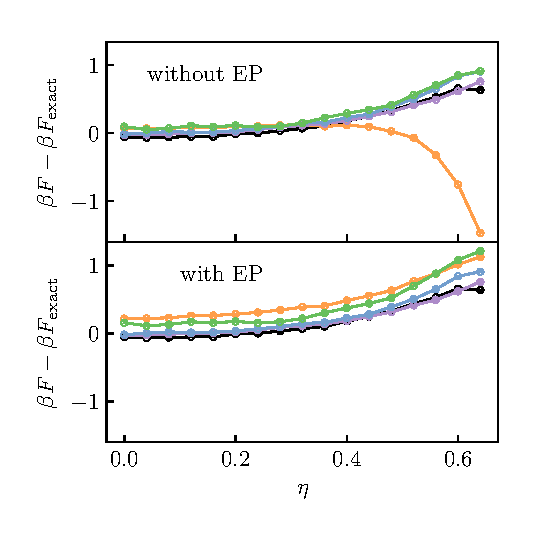
\includegraphics[width=0.9\linewidth,outer]{ep-n7}
  \caption[Errors in EP]{
    Error in the free energy evaluated with analytic methods (described in text) for the five $n = 7$ structures in Fig.\ \ref{fig:packings}.
    The exact result is taken from thermodynamic integration.
    The orange curve is for broken five-fold symmetry (spindle intact), thermal fluctuations very easily create overlaps.
  }
  \label{fig:ep-n7}
\end{SCfigure}

To go beyond this approximation we will approximate the geometry of hard sphere interactions to leading order; in effect, this models the boundary conditions as a polyhedron.
Next, we will use expectation propagation, a technique from Bayesian inference, to evaluate the integral on the resulting polyhedron.

\section{Polyhedral approximation}

We have a bond-distance space $\vec{x} \in \mathbb{R}^q$, $m = q$ constraints (minimally constrained for now) and $n(n-1)/2 - m$ potential interactions not already covered by the limits of integration.
We approximate this by measuring the distances not covered by the limits of integration and expanding them to linear order
\begin{equation}
  \Delta_{ij}(\vec{x})
  \simeq
  \Delta_{ij}(\vec{x}^*)
  + \left. \nabla \Delta_{ij} \right|_{\vec{x}^*} \cdot \Delta \vec{x}
  + \mathcal{O}(\Delta \vec{x}^2)
\end{equation}
and determine at this level of expansion the values of $\vec{x}$ where $\Delta_{ij} > \sigma$.
This is expressed as the inequality
\begin{equation}
  \Delta_{ij}(\vec{x}^*)
  + \left. \nabla \Delta_{ij} \right|_{\vec{x}^*} \cdot \Delta \vec{x}
  > \sigma
\end{equation}
to leading order where $\vec{c}_k = \nabla \Delta_{a_k,b_k}$.
This corresponds to assigning the half space constraint
\begin{equation}
  \vec{c}_k \cdot \Delta \vec{x} \in [\sigma - \Delta_{a_k,b_k}, \infty].
\end{equation}
The combination of half spaces and the cubic limits \eqref{?} describes a polyhedron in phase space, so this is a polyhedral approximation.
Similar approximations have been made for hard sphere free energy calculations in the crystal \cite{RadinPRL2005,KochPRE2005} and related systems \cite{LeoniPRL2017}, where this approximation becomes exact at very high densities approaching close packing.

Our partition function becomes an integral of the cavity function, in the exponential family, over a polyhedron.
Besides the simple one dimensional case few exact calculations are possible.
We will use an approximate method from Bayesian inference: expectation propagation.

\section{Expectation propagation}

Inspired by the Harmonic approximation where the energy is expanded to second order, we will attempt to approximate the basin probability distribution as a Gaussian.
We write this approximate probability distribution as
\begin{equation}
  q(\vec{x}) = Z \mathcal{N}(\vec{x}; \vec{\mu}, \vec{\Sigma}).
\end{equation}
where we have kept it unnormalised for convenience (so it is not strictly a distribution): our goal is to determine $Z$.
The moments of the Gaussian $\vec{\mu}, \vec{\Sigma}$ will be determined alongside $Z$, giving the evaluation of $I$ through \eqref{eq:rotation-metric-perturbations}.
Note that in the Bayesian inference literature $p(\vec{x}) \sim \mathcal{P}$ would be called the posterior distribution.

Consider the free energy difference between the true and approximate distribution
\begin{equation}
  \Delta F
  =
  - \int p(\vec{x})
  \ln{\left( \frac{q(\vec{x})}{p(\vec{x})} \right)} \, d\vec{x}.
\end{equation}
This would be the Kullback-Leibler divergence in information theory, a measure of information loss from using an approximate distribution.
It is identical to a free energy difference in the physics literature, and it is straightforward to prove that it is only zero when $p = q$ \cite{MerminPR1965, EvansAP1979}.
It is schematically identical to the proof of the uniqueness of the equilibrium free energy.

$\Delta F = 0$ is impossible unless $p$ is also Gaussian, however by minimising $\Delta F$ we can optimise the $q$ distribution to minimise the approximation error.
It is straightforward to show that for distributions in the exponential family this corresponds to matching the moments of $q$ and $p$ \cite{Minka2001,MinkaUAI2001,Rasmussen2006,Cunningham2011}.
This is still intractable however, matching moments is identical to setting the distributions to one another.
However, an approximate technique expectation propagation matches the moments of marginal distributions has been shown to approximate this well \cite{Minka2001,MinkaUAI2001,Rasmussen2006,Cunningham2011}.
This approximation was inspired by the cavity method of spin glasses (unrelated to the cavity distribution), for application to approximate Bayesian inference problems.

Our exposition of the EP method closely follows \cite{Cunningham2011}.

We start by noting that the true probability distribution, which includes the limits of integration, can be expressed as the product of distributions
\begin{equation}
  p(\vec{x})
  = y^{(n)}(\vec{x}) \prod_{i=1}^{m} t_i (x_i)
\end{equation}
where the $t_i$ functions represent the constraints \eqref{??} and \eqref{??}.
The EP algorithm constructs projections in each of these constraints to match moments along, a natural decomposition involves writing the approximate distribution in terms of tile distributions $\tilde{t}_i$
\begin{equation}
  q(\vec{x})
  = p_0(\vec{x}) \prod_{i=1}^{m} \tilde{t}_i (x_i)
  = p_0(\vec{x}) \prod_{i=1}^{m} \tilde{Z}_i \mathcal{N}(\vec{x}; \tilde{\mu}_i, \tilde{\sigma}_i^2)
\end{equation}
with projected values
\begin{subequations}
  \begin{align}
    x_i &= \vec{c}_i \cdot \vec{x} \\
    \mu_i &= \vec{c}_i \cdot \vec{\mu}
  \end{align}
\end{subequations}
for $i \in \{1,\cdots,m\}$.
From \eqref{eq:combined-normals} and \eqref{eq:biased-normal} we have
\begin{equation}
  \begin{split}
    q(\vec{x}) &=
    Z_0
    p_0(\vec{x})
    \mathcal{N}(\vec{x}; \vec{\Sigma} \cdot \vec{\nu}, \vec{\Sigma}) \\
    &=
    Z_0
    \exp{\left( \frac{\vec{a} \cdot \vec{\Sigma} \cdot \vec{a}}{2} - \vec{a} \cdot \vec{\Sigma} \cdot{\vec{\nu}} \right)} \;
    \mathcal{N}(\vec{x}; \vec{\Sigma} \cdot (\vec{\nu} - \vec{a}), \vec{\Sigma})
  \end{split}
\end{equation}
where $\vec{\Sigma}, \vec{\nu}, Z_0$ are given by \eqref{eq:combined-normals-sigma}, \eqref{eq:combined-normals-nu} and \eqref{eq:combined-normals-Z} respectively.
We thus have
\begin{subequations}
  \begin{align}
    \vec{\mu} &= \vec{\Sigma} \cdot (\vec{\nu} - \vec{a})
    \\
    Z &= Z_0
    \exp{\left( \frac{\vec{a} \cdot \vec{\Sigma} \cdot \vec{a}}{2} - \vec{a} \cdot \vec{\Sigma} \cdot \vec{\nu} \right)}
    \\
    Z_0 &=
    \sqrt{ (2\pi)^{n-m} \det{\vec{\Sigma}} }
    \;
    \exp{\left( \frac{\vec{\nu} \cdot \vec{\Sigma} \cdot \vec{\nu}}{2} \right)}
    \prod_{i=1}^m
    \left(
    \frac{\tilde{Z}_i}{\sqrt{ \tilde{\sigma}_i^2 }}
    \exp{\left(-\frac{\tilde{\nu}_i \tilde{\mu}_i}{2}\right)}
    \right)
  \end{align}
\end{subequations}
We marginalise the full probability distribution along one direction to obtain the cavity distribution
\begin{equation}
  q^{\setminus i}(\vec{x}) =
  \frac{\tilde{Z}_i}{Z} \frac{q(\vec{x})}{\tilde{t}_i(x_i)}
  =
  \frac
      {\mathcal{N}(\vec{x}; \vec{\mu}, \vec{\Sigma})}
      {\mathcal{N}(x_i; \tilde{\mu}_i, \tilde{\sigma}_i^2)}.
\end{equation}
This particular normalisation is chosen such that
\begin{equation}\label{eq:approximate-zeroth-moment}
  \int_{\mathbb{R}^n} q^{\setminus i}(\vec{x}) \tilde{t}_i(x_i) \, d\vec{x} =
  \tilde{Z}_i \int_{\mathbb{R}^n} \mathcal{N}(\vec{x}; \vec{\mu}, \vec{\Sigma}) \, d\vec{x} =
  \tilde{Z}_i.
\end{equation}
Integrating this cavity over the orthogonal affine space gives
\begin{equation}
  \begin{split}
    q_{\setminus i}(x_i) &\equiv
    \int_{\mathbb{R}^n \setminus \vec{c}_i} q^{\setminus i} (\vec{x}_{\setminus i}; x_i) \, d\vec{x}_{\setminus i} \\
    &= \frac{1}{\mathcal{N}(x_i; \tilde{\mu}_i, \tilde{\sigma}_i^2)}
    \int_{\mathbb{R}^n \setminus \vec{c}_i} \mathcal{N}(\vec{x}; \vec{\mu}, \vec{\Sigma}) \, d\vec{x}_{\setminus i} \\
    &=
    \frac
        {\mathcal{N}(x_i; \mu_i, \vec{c}_i \cdot \vec{\Sigma} \cdot \vec{c}_i)}
        {\mathcal{N}(x_i; \tilde{\mu}_i, \tilde{\sigma}_i^2)} \\
    &=
        \sqrt{ \frac{\tilde{\sigma}_i^2}{\vec{c}_i \cdot \vec{\Sigma} \cdot \vec{c}_i} }
        \exp{\left( -\frac{(x_i - \mu_i)^2}{2 \vec{c}_i \cdot \vec{\Sigma} \cdot \vec{c}_i} +
          \frac{(x_i - \tilde{\mu}_i)^2}{2 \tilde{\sigma}_i^2} \right)} \\
    &=
        \sqrt{ \frac{\sigma_{\setminus i}^2 + \tilde{\sigma}_i^2}{\sigma_{\setminus i}^2} }
        \exp{\left(
          - \frac{(x_i - \mu_{\setminus i})^2}{2 \sigma_{\setminus i}^2}
          + \frac{1}{2}
          \frac{(\mu_{\setminus i} - \tilde{\mu}_i)^2}{\sigma_{\setminus i}^2 + \tilde{\sigma}_i^2}
          \right)} \\
     &= Z_{\setminus i} \, \mathcal{N}(x_i; \mu_{\setminus i}, \sigma_{\setminus i}^2)
  \end{split}
\end{equation}
where we completed the square in the penultimate step using the cavity parameters: \cite{Rasmussen2006,Cunningham2011}
\begin{align}
  Z_{\setminus i}
  &=
  \sqrt{2 \pi (\sigma_{\setminus i}^2 + \tilde{\sigma}_i^2)}
  \exp{\left(
    \frac{1}{2}
    \frac{(\mu_{\setminus i} - \tilde{\mu}_i)^2}{\sigma_{\setminus i}^2 + \tilde{\sigma}_i^2}
    \right)}
        \\
  \sigma_{\setminus i}^2 &= \left(
  \frac{1}{\vec{c}_i \cdot \vec{\Sigma} \cdot \vec{c}_i} - \frac{1}{\tilde{\sigma}_i^2}
  \right)^{-1} \\
  \mu_{\setminus i} &= \sigma_{\setminus i}^2 \left(
  \frac{\mu_i}{\vec{c}_i \cdot \vec{\Sigma} \cdot \vec{c}_i} - \frac{\tilde{\mu}_i}{\tilde{\sigma}_i^2}
  \right).
\end{align}
Note that the cavity distribution is the properly normalised quantity $q_{\setminus i}(x_i) / Z_{\setminus i}$.
The exact zeroth cavity moment is found via \cite{Cunningham2011}
\begin{equation}\label{eq:exact-zeroth-moment}
  \frac{\hat{Z}_i}{Z_{\setminus i}} =
  \frac{1}{Z_{\setminus i}}
  \int_{\mathbb{R}} q_{\setminus i}(x_i) t_i(x_i) \, dx_i
  = \frac{1}{2} \left( \erf{\beta_i} - \erf{\alpha_i} \right)
\end{equation}
where we have used the shorthand
\begin{align}
  \alpha_i &= \frac{l_i - \mu_{\setminus i}}{\sqrt{2} \sigma_{\setminus i}} \\
  \beta_i &= \frac{u_i - \mu_{\setminus i}}{\sqrt{2} \sigma_{\setminus i}}.
\end{align}
The above relations are numerically unstable in the limit of small $\sigma_i^2 - \tilde{\sigma}_i^2$, so we have to handle this case by Taylor expansion:
\begin{align}
  q_{\setminus i}(x_i) &=
  \frac{
    \mathcal{N}(x_i; \vec{c}_i \cdot \vec{\mu}, \vec{c}_i \cdot \vec{\Sigma} \cdot \vec{c}_i)
  }{
    \mathcal{N}(x_i; \tilde{\mu}_i, \tilde{\sigma}_i^2)
  }
  =
  \frac{\mathcal{N}(x_i; \mu_i, \sigma_i^2)}{
    \mathcal{N}(x_i; \tilde{\mu}_i, \tilde{\sigma}_i^2)
  }
  \nonumber \\ &=
  \exp{\left(-a_i x_i
    - \frac{a_i^2 \sigma_i^2}{2}
    + a_i \mu_i
    \right)}
  \frac{\mathcal{N}(x_i; \mu_i + a_i \sigma_i^2, \sigma_i^2)}{
    \mathcal{N}(x_i; \tilde{\mu}_i, \tilde{\sigma}_i^2)
  }
\end{align}
where $a_i = \vec{a} \cdot \vec{c}_i$, giving
\begin{align}
  \hat{Z}_i
  =&
  \int_{\mathbb{R}} q_{\setminus i}(x_i) t_i(x_i) \, dx_i
  \nonumber \\ =&
  \sqrt{ \frac{\tilde{\sigma}_i^2}{\vec{c}_i \cdot \vec{\Sigma} \cdot \vec{c}_i} }
  \int_0^{\delta_i}
  \exp{\left( -\frac{(x_i - \mu_i)^2}{2 \vec{c}_i \cdot \vec{\Sigma} \cdot \vec{c}_i} +
    \frac{(x_i - \tilde{\mu}_i)^2}{2 \tilde{\sigma}_i^2} \right)} \, dx_i
  \nonumber \\ =&
  \sqrt{ \frac{\tilde{\sigma}_i^2}{\vec{c}_i \cdot \vec{\Sigma} \cdot \vec{c}_i} }
  \exp{\left(
    - \frac{a_i^2 \sigma_i^2}{2}
    + a_i \mu_i
    \right)}
  \nonumber \\ &
  \times \int_0^{\delta_i}
  \exp{\left( -\frac{(x_i - (\mu_i + a_i \sigma_i^2))^2}{2 \vec{c}_i \cdot \vec{\Sigma} \cdot \vec{c}_i} +
    \frac{(x_i - \tilde{\mu}_i)^2}{2 \tilde{\sigma}_i^2} - a_i x_i \right)} \, dx_i.
\end{align}
Matching moments between \eqref{eq:approximate-zeroth-moment} and \eqref{eq:exact-zeroth-moment} gives us
\begin{equation}
  \tilde{Z}_i = \frac{\hat{Z}_i}{Z_{\setminus i}}
  \sqrt{2 \pi (\sigma_{\setminus i}^2 + \tilde{\sigma}_i^2)}
  \exp{\left(
    \frac{1}{2}
    \frac{(\mu_{\setminus i} - \tilde{\mu}_i)^2}{\sigma_{\setminus i}^2 + \tilde{\sigma}_i^2}
    \right)}.
\end{equation}
We calculate $\hat{Z}_i / Z_{\setminus i}$ from \eqref{eq:exact-zeroth-moment} and then obtain the partition function from
\begin{equation}
  \begin{split}
    \log{\tilde{Z}_i}
    =
    \frac{1}{2} \left(
    \log{(2\pi)} +
    \log{(\sigma_{\setminus i}^2 + \tilde{\sigma}_i^2)} +
    \frac{(\mu_{\setminus i} - \tilde{\mu}_i)^2}{\sigma_{\setminus i}^2 + \tilde{\sigma}_i^2}
    \right.&
    \\
    \left.
    + \log{\left(\frac{\erf{\beta_i} - \erf{\alpha_i}}{2}\right)}
    \right)&
  \end{split}
\end{equation}
Giving the final partition function:
\begin{equation}
  \begin{split}
    \log{Z}
    =&
    \frac{1}{2} \left(
    (n-m) \log{2\pi}
    + \log\det{\vec{\Sigma}}
    + \vec{\nu} \cdot \vec{\Sigma} \cdot \vec{\nu}
    \right)
    \\ &
    + \sum_{i=1}^m \left(
    \log{\tilde{Z}_i}
    - \frac{1}{2}
    \left(
    \log{\tilde{\sigma}_i^2}
    + \tilde{\nu}_i \tilde{\mu}_i
    \right)
    \right)
  \end{split}
\end{equation}
where we have either
\begin{align}
  & \log{\tilde{Z}_i}
  - \frac{1}{2}
  \left(
  \log{\tilde{\sigma}_i^2}
  + \tilde{\nu}_i \tilde{\mu}_i
  \right)
  \nonumber \\ =&
  \frac{1}{2} \left(
  \log{(2\pi)} +
  \log{(\sigma_{\setminus i}^2 + \tilde{\sigma}_i^2)} +
  \frac{(\mu_{\setminus i} - \tilde{\mu}_i)^2}{\sigma_{\setminus i}^2 + \tilde{\sigma}_i^2}
  \right.
  \nonumber \\ & \qquad
  \left.
  + \log{\left(\frac{\erf{\beta_i} - \erf{\alpha_i}}{2}\right)}
  - \log{\tilde{\sigma}_i^2}
  - \tilde{\nu}_i \tilde{\mu}_i
  \right)
  \nonumber \\ =&
  \frac{1}{2} \left(
  \log{(2\pi)} +
  \log{\left(\frac{\sigma_{\setminus i}^2 + \tilde{\sigma}_i^2}{\tilde{\sigma}_i^2}\right)}
  + \frac{(\mu_{\setminus i} - \tilde{\mu}_i)^2}{\sigma_{\setminus i}^2 + \tilde{\sigma}_i^2}
  \right.
  \nonumber \\ & \qquad
  \left.
  - \tilde{\nu}_i \tilde{\mu}_i
  + \log{\left(\frac{\erf{\beta_i} - \erf{\alpha_i}}{2}\right)}
  \right)
  \nonumber \\ =&
  \frac{1}{2} \left(
  \log{(2\pi)} +
  \log{(1 + \tilde{\tau}_i \sigma_{\setminus i}^2)}
  + \frac{\tilde{\tau}_i \mu_{\setminus i}^2 - 2\tilde{\nu}_i \mu_{\setminus i} - \tilde{\nu}_i^2 \sigma_{\setminus i}^2}
  {1 + \tilde{\tau}_i \sigma_{\setminus i}^2}
  \right.
  \nonumber \\ & \qquad
  \left.
  + \log{\left(\frac{\erf{\beta_i} - \erf{\alpha_i}}{2}\right)}
  \right)
\end{align}
or for small $\sigma_i^2 - \tilde{\sigma_i^2}$ we use
\begin{equation}
  \begin{split}
    &
    \log{\tilde{Z}_i}
    - \frac{1}{2}
    \left(
    \log{\tilde{\sigma}_i^2}
    + \tilde{\nu}_i \tilde{\mu}_i
    \right)
    \\ =&
    \frac{1}{2} \left( -\log{\vec{c}_i \cdot \vec{\Sigma} \cdot \vec{c}_i} \right)
    + a_i \mu_i
    - \frac{a_i^2 \sigma_i^2}{2}
    - \frac{\tilde{\nu}_i \tilde{\mu}_i}{2}
    \\ & + 
    \log{\left(
      \int_0^{\delta_i}
      \exp{\left( -\frac{(x_i - (\mu_i + a_i \sigma_i^2))^2}{2 \vec{c}_i \cdot \vec{\Sigma} \cdot \vec{c}_i} +
        \frac{(x_i - \tilde{\mu}_i)^2}{2 \tilde{\sigma}_i^2} -a_i x_i \right)} \, dx_i
      \right)}.
  \end{split}
\end{equation}

\begin{SCfigure}
  \includegraphics[width=0.9\linewidth,outer]{ep-errors}
  \caption[Errors in expectation propagation for integration over a triangle]{
    Expectation propagation error for integrating a simple potential over a triangle with field $\vec{A} = (a, a)$.
  }
  \label{fig:ep-errors}
\end{SCfigure}

\section{Worked example: area of a triangle}

As a simple example we consider the area of a triangle as a unit square.
We can write this area as the integral over a box
\begin{equation}
  A = \int_0^1 \int_0^1 \Theta(1 - x - y) \, dx dy
  = \frac{1}{2}
\end{equation}
where $\Theta(\cdot)$ is the Heaviside function.
The exact result is fairly trivial, but as it can also be evaluated using expectation propagation we can use this as a worked example and to justify the method.
EP gives an area $A \simeq 0.515$ for an error of about 3\%.

\begin{SCfigure}
  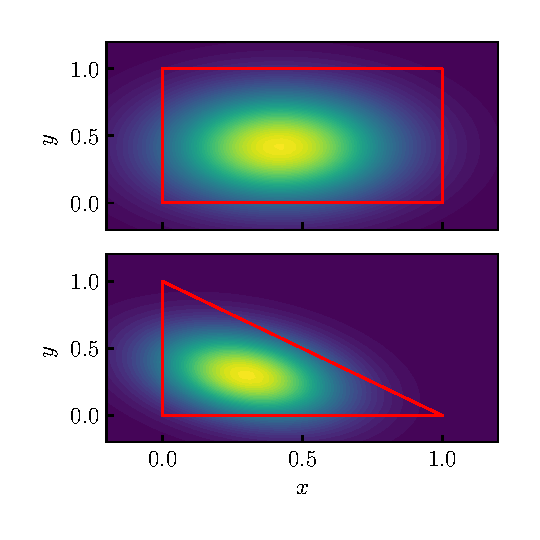
\includegraphics[width=0.9\linewidth,outer]{ep-pdf}
  \caption[Approximate probability distribution assumed in blah]{
    Sketch of integration scheme proposed as generalisation of harmonic approximation: true distribution modelled as a Gaussian.
    We use expectation propagation as criteria for optimal parameters for the Gaussian.
    In each panel the boundary of the integration area is indicated by red lines.
    For a field $\vec{A} = \{1,1\}$.}
\end{SCfigure}

This is a pathological case: no potential, pure geometry.
We expect the error to improve when integrating functions over the box.
We generalise the integral to
\begin{equation}
  Z = \int_0^1 \int_0^1 \Theta(1 - x - y) e^{-A_x x - A_y y} \, dx dy
\end{equation}
with the results shown in Fig.\ \ref{fig:ep-errors}.
We see that the effective Gaussian is skewed by the additional constraint, stretching to approximate the triangular shape of the boundary.

\ifdefined\includebibliography
  \newgeometry{margin=1in}
  \printbibliography
\fi

\end{document}
